This chapter describes the process by which we designed and conducted a user study to evaluate our metro maps against unstructured RSS feed readers. Results and implications of this study are discussed, with full data available in Appendix \ref{sec:evalresults}. The two metro maps used for the study have been included in Appendix  \ref{sec:evalmaps}.

\section{Scoping the Experiments}

Typically, information retrieval tools can be evaluated in terms of  accuracy and other quantifiable metrics against a canonical labelled dataset. Our system is less amenable to such evaluation due to the lack of existing datasets. The extensive user study conducted by \cite{GeneratingInformationMaps} evaluated four distinct aspects of their metro map system; (1) accuracy of the algorithm's document selection in respect to a query; (2) user fact retrieval time; (3) user understanding at a macro level; and (4) task performance of users with a Metro Map versus an unstructured list.

For our system, the first aspect (accuracy of retrieval for queries) is not of interest, because the maps are not query-based or selected from a large fixed corpus with a reasonable likelihood of Type II errors. The second and third, while relevant to our system, do not effectively capture the spirit of its intended purpose. Our metro maps are not designed for search tasks; if a user has a specific question about an article in a metro map, they will most likely still have to open and read the article itself for the answer. 

The maps the generated by the system exist to help the user form high-level connections between topics and to make sense of those they do not understand. A search task would therefore have to ask artificially simple questions in order for the answers to be derivable using the maps alone, and this would not be representative of typical news consumption tasks.

The final aspect of the \citeauthor{GeneratingInformationMaps} study was therefore chosen as the focus of this evaluation. The goal of the experiments was to determine whether the structure of the metro maps alone provided a better overview to news content than a traditional RSS feed view. This question was answered by using \possessivecite{TowardsAnOptimalResolutionToInformationOverload} dimensions of information overload to choose two perspectives to evaluate:

\begin{itemize}
	\item Users' perceptions of \textbf{information quantity}. \par
		As information overload is based partially on readers' intrinsic estimations of quantity, we examined the effect that varying information format has on these estimations.
	\item The \textbf{contextual quantity} of our maps, as measured by task performance. \par
		We conducted an experiment similar to that of \cite{scattergather}, measuring the effect of varying information format on the breadth and depth of users' topic recollection.
\end{itemize}

\section{Experimental Hypotheses}

Considering perception and performance as our two separate measures of information overload, we developed the following hypotheses to be tested in two corresponding experiments:

\begin{hyp}[\ref{hyp:eq:estimation}]
\label{hyp:estimation}
Users' estimates of the number of articles in a metro map are lower than their estimates of the same number of articles when displayed in a list form.
\end{hyp}
\vspace{-0.6cm}
\begin{align*}
	H_{0}(\ref{hyp:estimation}) &: \mu{E_{map}} = \mu{E_{list}} \\
	H_{1}(\ref{hyp:estimation}) &: \mu{E_{map}} < \mu{E_{list}} \numberthis
	\label{hyp:eq:estimation}
\end{align*}

\begin{hyp}[\ref{hyp:eq:index}]
\label{hyp:index}
Users recall a higher number of topics after using a metro map representation than after using the RSS feed list view.
\end{hyp}
\vspace{-0.6cm}
\begin{align*}
	H_{0}(\ref{hyp:index}) &: \mu{T_{map}} = \mu{T_{list}} \\
	H_{1}(\ref{hyp:index}) &: \mu{T_{map}} > \mu{T_{list}} \numberthis
	\label{hyp:eq:index}
\end{align*}

Where $\mu{E}_{map}$ and $\mu{E}_{list}$ are the mean estimate values for the number of articles contained within a map and list respectively, and $\mu{T}_{map}$ and $\mu{T}_{list}$ are the mean number of topics successfully recalled.

\section{Experimental Design}

In order to increase the number of subjects participating in each condition and control for individual variances in ability, both experiments were conducted within-groups. With each subject participating in both conditions (\textit{map} and \textit{list}), two corpora of news articles were required. Subjects were therefore assigned to one of four groups, with counterbalancing of both the order in which the conditions were conducted, and the order in which the two corpora were read (Table \ref{tab:experimentalgroups}.) Each group contained four participants.\\

\begin{table}[htbp!]
\centering
\begin{tabular}{|r|c|c|}
\hline
  & A, B & B, A\\
\hline
\textit{List}, \textit{Map} & (Group 1) \textit{List} A \textbf{then} \textit{Map} B & (Group 3) \textit{List} B \textbf{then} \textit{Map} A \\
\hline
\textit{Map}, \textit{List} & (Group 2) \textit{Map} A \textbf{then} \textit{List} B & (Group 4) \textit{Map} B \textbf{then} \textit{List} A \\
\hline
\end{tabular}
\caption{Participant groups} \label{tab:experimentalgroups}
\end{table}

\subsubsection{Participants}
In total, sixteen participants (four female, eight male, mean age = 21.8 years) enrolled in the study. All had perfect or corrected-to-perfect vision and hearing, and all were undergraduate students at the University of Bath. No participants were excluded on the basis of how much or how little news they consumed on a daily basis. Similarly, although it was recorded whether participants had previously used or currently use an RSS feed reader, this was not used as a selection criterion. 

Before starting the experiments, the purpose of the evaluation was explained, and each participant signed a copy of the standard consent form in Appendix \ref{sec:consent}. Afterwards, participants were debriefed and our hypotheses were explained to them.

\section{Methodology}

\subsection{Estimate Task} \label{task:est}

The first experiment was designed to test Hypothesis \ref{hyp:estimation}. Participants were exposed to both modalities for one minute, after which they estimated the number of articles they had been looking at. To prevent conscious or subconscious counting by participants during the second condition, it was only after exposure to the second set of articles that subjects were asked to estimate the number of articles in each.

\subsection{Index Task}

The second experiment, which was designed to test Hypothesis \ref{hyp:index}, placed a significantly greater cognitive load on  participants. This task is based on the evaluation of the Scatter/Gather Browser by \cite{scattergather}, which required participants to draw a topic index, or \textit{tree}, representing their understanding of topic structure within a corpus.

For each of the two conditions, participants first spent three minutes reading and exploring the news represented.\footnote{As this task was completed after the Estimate Task (Section \ref{task:est}), the total time spent interacting with the data was actually four minutes.} After the three minutes, the modality was minimised and the participants were given two minutes to write a topic index based on the news they had just read. An example topic index based on news in a different domain was shown before this task began to ensure participants knew what they were supposed to produce. Both datasets (and therefore all four conditions) contained 31 articles.

Finally, participants were asked to complete a Self-Assessment Manikin \citep{measuringemotion} to rate the pleasure (labelled from `unhappy' to `happy'), arousal (`calm' to `excited') and dominance (`not in control' to `in control') they felt as a result of completing the index task. This process was then repeated with the second modality and data set, according to the participant's grouping. The counterbalanced ordering of two conditions between groups controlled for the practice effect in this task.

\subsection{Variables}

The following section describes the independent variable in both studies, the dependent variables we measured, and the control variables which we either controlled through the design of the study or analysed as potential covariates.

\subsubsection{Independent Variables}

The independent variable in both experiments was the display modality; a nominal value which was either \textit{metro map} or \textit{list}. Participants completed the same tasks with both a metro map and a list modality, using a different news corpus for each.

\subsubsection{Dependent Variables}

\begin{itemize}
	\item\textbf{Article Estimate (Hypothesis \ref{hyp:estimation})} \par
		This is the raw estimate of the number of articles, and is measured on a ratio scale. 
	\item\textbf{Primary topics (Hypothesis \ref{hyp:index})} \par
		This is the number of `top-level' topics identified in a participant's index which are present in the corpus, measured on a ratio scale. If participants identified a single primary topic (e.g. `America'/ `The USA'), this top level of the index was ignored and primary topics were counted as those in the next level.
	\item\textbf{Topic index depth (Hypothesis \ref{hyp:index})} \par
		This is the maximum depth reached from any primary topic in a participant's index, measured on a ratio scale.
	\item\textbf{Total topics (Hypothesis \ref{hyp:index})} \par
		This is the total number of topics identified at all levels in a participant's index which are present in the corpus, measured on a ratio scale.
	\item\textbf{Self-Assessment Manikin (SAM) score (Hypothesis \ref{hyp:index})} \par
		The valence, arousal and dominance self-reported  by participants after completing the Index Task. These were measured on the 9-point scale variant, as shown by the arousal scale in Figure \ref{fig:9sam}.
\end{itemize}
\begin{figure}[htbp!]
	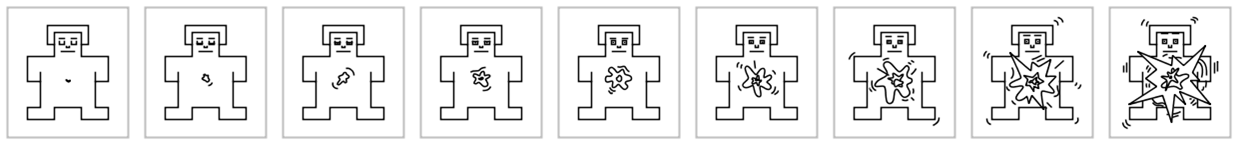
\includegraphics[width=\textwidth]{img/evaluation/dominance.png}
	\caption{The 9-point SAM scale representing arousal, from $calm$ to $excited$ \citep{measuringemotion}}
	\label{fig:9sam}
\end{figure}

\subsubsection{Control Variables}
The following are the participant characteristics and experimental conditions which were identified as potential covariates. Weekly news consumption, which we chose not to control through participant selection, was later examined as a influencing factor on performance.

\begin{itemize}
	\item\textbf{Level of formal education} \par
		It was expected that differing levels of formal education would impact the relative performance of participants, however all participants were undertaking the final year of an undergraduate degree, so we did not account for this as a covariate.
	\item\textbf{Weekly news consumption time} \par
		It was expected that participants who consume more news on average would perform uniformly better across both conditions, but as subjects participated in both conditions, we do not expect to need to account for this as a covariate. This variable was measured on a discrete scale of hours per week.
	\item\textbf{Topic Familiarity} \par
		Since all subjects participated in both conditions, each subject completed the \textit{metro map} condition with one set of articles and the \textit{list} condition with the other set. The two corpora (A and B) were extracted from the same RSS feed\footnote{The Guardian, US News, week commencing 20/03/2017.} within the same week, to ensure background knowledge wouldn't confound performance between A and B.
\end{itemize}

\section{Results and Discussion}

A complete set of results for the following tests is available in Appendix \ref{sec:evalresults} (Hypothesis \ref{hyp:estimation}: Table \ref{res:estimate}, Hypothesis \ref{hyp:index}: Table \ref{res:index}, tests for normality: Table \ref{res:sw}, correlations: Tables \ref{res:hourscorrelation} -  \ref{res:samcomposites}), with raw data in Section \ref{sec:evalraw}.

The use of one-tailed tests, even in the case of clear directional hypotheses, is controversial and may be seen as insufficiently conservative. However, for exploratory research like this which is necessarily limited in statistical power, we hope it is justified as exposing effects which seem promising. Future studies could test these same hypotheses more thoroughly.

\subsection{Testing Hypothesis \ref{hyp:estimation}: Estimate Task}

Our first hypothesis predicted that users' estimates for the number of articles represented on a map would be lower than their estimates of the same number of articles shown in the form of a list. A paired-samples $t$-test was conducted to compare estimates for the \textit{map} and \textit{list} conditions. Data was screened for violation of the following assumptions before the test was performed:
\vspace{-0.2cm}
\begin{itemize}[itemsep=0.05em,leftmargin=0.7cm]
	\item \textbf{Continuous Measurement}: Both estimates were measured on a continuous scale.
	\item \textbf{Independence}: Participants' estimates were independent, as the experiment placed them in isolation.
	\item \textbf{Outliers}: There were no outliers in either of the estimates.
	\item \textbf{Normality}: The normality assumption was tested with the Shapiro-Wilk test on \textit{map estimate} (W=0.881, df=16, $p$=.080) and \textit{list estimate}  (W=0.954, df=16, $p$=.559). These results suggest normality is a reasonable assumption for the data.
\end{itemize}

Figure \ref{fig:estimate} shows the means for each condition split by corpus. Although the mean estimates for Corpus A were lower, this difference was not significant.

\begin{figure}[htbp!]
	\centering
	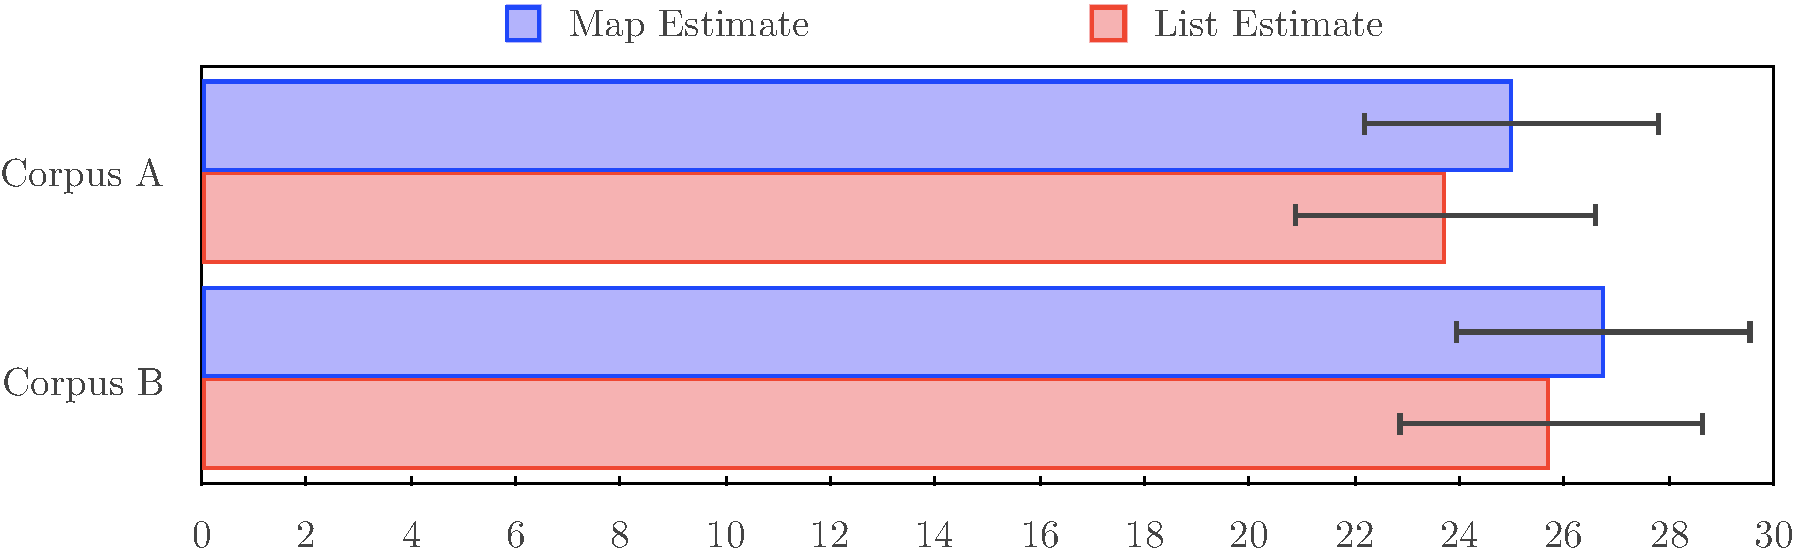
\includegraphics[width=.95\textwidth]{img/evaluation/estimate.pdf}
	\caption{Comparison of \textit{Map} and \textit{List} estimates between the two corpora}
	\label{fig:estimate}
\end{figure}

The results of the $t$-test suggest there was no significant difference in estimates between the map (M=24.75, SD=7.188) and list (M=25.88, SD=6.820) conditions; $t$(15)=-0.504, $p$=.311 (one-tailed, $\alpha=.05$), providing insufficient evidence to reject $H_0$. We conclude that there is no significant difference between participants' perceptions of information quantity on the basis of modality alone.

\subsection{Testing Hypothesis \ref{hyp:index}: Index Task}

Our second hypothesis predicted that users would identify more topics in their index after using the map than after using the list. A second paired-samples $t$-test was conducted to compare the number of topics produced during the \textit{map} and \textit{list} conditions.

As in the previous test, there was no missing data, and data was screened for violation of measurement level, independence, outliers and normality (\textit{map topics}: W=0.958, df=16, $p$=.633,  \textit{list topics}: W=0.917, df=16, $p$=.152) as before. Figure \ref{fig:index} verifies that there was no significant difference in total index topics produced between corpora A and B.

\begin{figure}[htbp!]
	\centering
	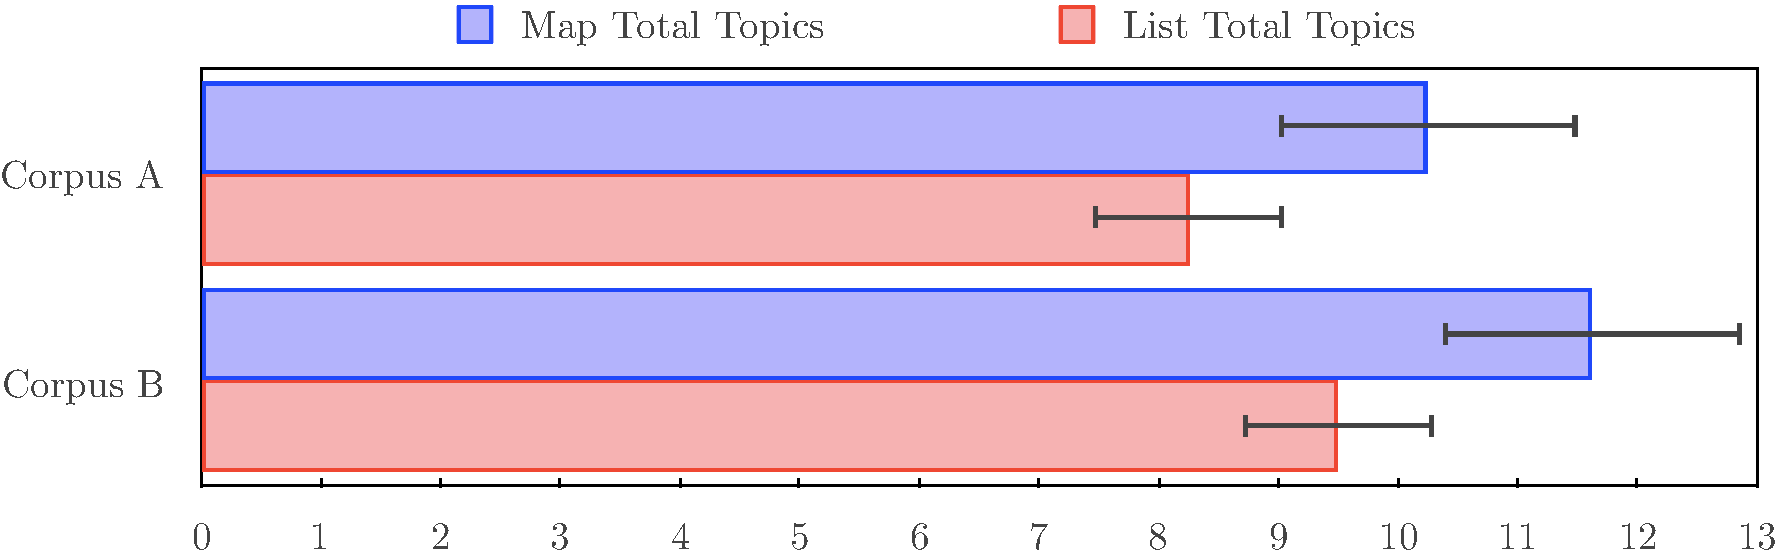
\includegraphics[width=.9\textwidth]{img/evaluation/index.pdf}
	\caption{Comparison of \textit{Map} and \textit{List} total topics between the two corpora}
	\label{fig:index}
\end{figure}

The results of the test did show a significant difference in total topics produced in the map (M=10.94, SD=4.389) and list (M=8.88, SD=2.156) conditions; $t$(15)=2.254, $p$=.20 (one-tailed, $\alpha=.05$), providing sufficient evidence to reject $H_0$. Since these results supported our hypothesis, we conducted a second round of tests in an attempt to determine whether the additional topics produced by users with metro maps was due to additional breadth or depth of their news recall. The additional dependent variables we measured during the index task were \textit{primary topics} (topics at the highest level of the index, analogous to breadth of recall) and \textit{topic depth} (the maximum depth reached in an index). 

Two further paired-samples $t$-tests were therefore conducted to compare the respective breadths and depths of participants' indexes between the two modalities (Figure \ref{fig:depthbreadth}).

\begin{figure}[htbp!]
\centering
\begin{minipage}{.5\textwidth}
  \centering
  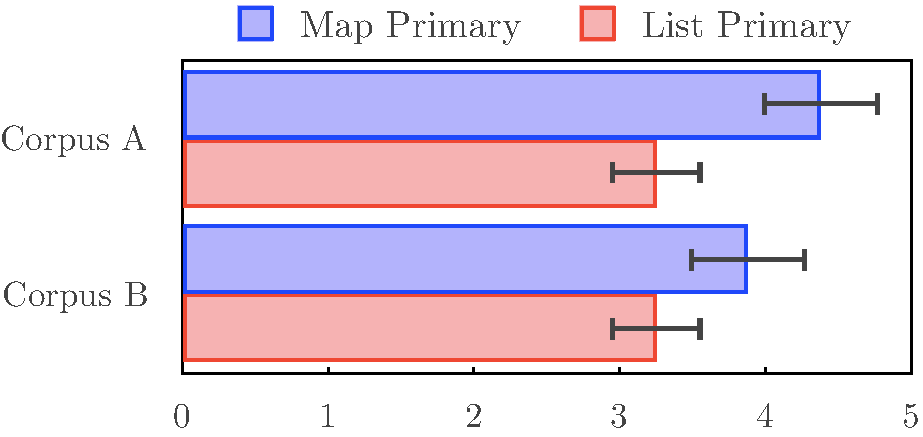
\includegraphics[height=.48\linewidth]{img/evaluation/primary.pdf}
  \end{minipage}%
\begin{minipage}{.5\textwidth}
  \centering
  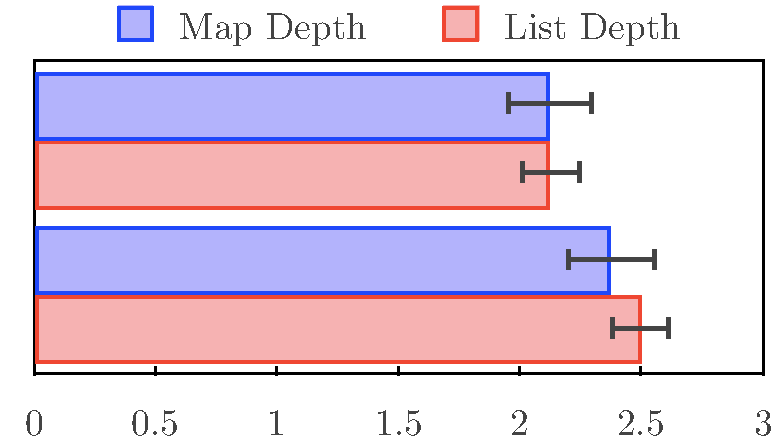
\includegraphics[height=.48\linewidth]{img/evaluation/depth.pdf}
\end{minipage}
	\caption{Comparison of \textit{Map} and \textit{List} topic breadth and depth between the two corpora}
  \label{fig:depthbreadth}
\end{figure}

These tests showed no significant difference between map index depth (M=2.25, SD=0.577) and list index depth (M=2.31, SD=0.602); $t$(15)=-0.368, $p$=.359 (one-tailed, $\alpha=.05$), however, they did show a significant difference between map primary topics (M=4.19, SD=1.607) and list primary topics (M=3.25, SD=1.125) conditions; $t$(15)=1.996, $p$=.032, at the same significance level.

The implication of this result is that the additional topics participants were able to recall in the \textit{map} condition were due to increased recall of the breadth of the news they had read, rather than increased in-depth recall of any particular topics.

\subsection{The Effects of Weekly News Consumption}

The average weekly news consumption of participants was a factor we identified as a potential influencer of task performance. Although our within-subjects design would have controlled any confounding effects, we analysed the Pearson correlation of this variable with several of our dependent variables to identify any unexpected correlations.

There was no significant correlation between average weekly news consumption time and participants' estimates of the number of articles on the map or in the list.

In the index task, news consumption was similarly correlated with total index topics for both the \textit{map} ($r$=0.541, $p$=.031) and \textit{list} ($r$=0.573, $p$=.020) conditions. As expected, high news consumption positively influenced performance. The strongest correlation with news consumption however, was with the index depth in the \textit{map} condition ($r$=0.606, $p$=.013). This, in contrast to the lack of any significant correlation in the \textit{list} condition suggests that in drawing the users' focus to a wider breadth of topics, metro maps may sacrifice their understanding of topic depth.

\subsection{Self-Assessment Manikin Scores}

The three dimensions of affect measured by the Self-Assessment Manikin \citep{measuringemotion} are pleasure (P), arousal (A), and dominance (D). \cite{emotionbasedtheory} classified every combination of high and low scores for each dimension, resulting in the following octants:

\begin{table}[htbp!]
\centering
\begin{tabular}{lllll}
\textit{Exuberant} & (+P, +A, +D) & vs. & \textit{Bored} & ($-$P, $-$A, $-$D) \\
\textit{Relaxed} & (+P, $-$A, +D) & vs. & \textit{Anxious} & ($-$P, +A, $-$D) \\
\textit{Hostile} & ($-$P, +A, +D) & vs. & \textit{Docile} & (+P, $-$A, $-$D) \\
\textit{Distainful} & ($-$P, $-$A, +D) & vs. & \textit{Dependent} & (+P, +A, $-$D)
\end{tabular}
\end{table}

Although these were proposed as a taxonomy for human personality and temperaments, we expect the labels to generalise to emotional responses composed of the same three dimensions of affect, as measured using SAM scores.

In our analysis of the correlations between the three SAM dimensions, we found participants' pleasure to be to highly correlated to the levels of dominance they felt using the modality (\textit{Map}: $r$=0.773, $p<$.001; \textit{List}: $r$=0.685, $p$=.003) but uncorrelated with the level of arousal they reported. This suggests that enjoyment of both modalities is based on whether or not the participants felt in control while using them.

There was no correlation between the two modalities in terms of pleasure or dominance, but there was a correlation between \textit{map} arousal and \textit{list} arousal ($r$=0.646, $p$=.007), which suggests that arousal may be a function of enjoyment of news content itself and unrelated to the specific modality.

Due to the strong positive correlations between pleasure and dominance observed in SAM scores for both conditions, four of \citeauthor{emotionbasedtheory}'s octants are less relevant to our results. We can therefore restrict the set of typical emotional responses to the \textit{map} and \textit{list} conditions to tuples where sign(P) = sign(D):

\begin{table}[htbp!]
\centering
\begin{tabular}{lllll}
\textit{Exuberant} & (+P, +A, +D) & vs. & \textit{Bored} & ($-$P, $-$A, $-$D) \\
\textit{Relaxed} & (+P, $-$A, +D) & vs. & \textit{Anxious} & ($-$P, +A, $-$D) \\
\end{tabular}
\end{table}

When pleasure and dominance are both high, it is not immediately obvious which emotional response is the desirable outcome between exuberance and relaxation. Taking each participant's exuberance as (P+A+D) and their relaxation as (P$-$A+D) and correlating these composite variables with the results of the index task, a strong link emerges between exuberance and total topics produced in the \textit{map} condition ($r$=0.753, $p$=.001), as shown in Figure \ref{fig:exuberance}. No such correlation exists with relaxation in the \textit{map} condition, or with either of these two variables in the \textit{list} condition.\\

\begin{figure}[htbp!]
\centering
\begin{minipage}{.5\textwidth}
  \centering
  \includegraphics[width=.9\linewidth]{img/evaluation/listexuberance.pdf}
  \end{minipage}%
\begin{minipage}{.5\textwidth}
  \centering
  \includegraphics[width=.9\linewidth]{img/evaluation/mapexuberance.pdf}
\end{minipage}
	\caption{Comparison of correlations between index topics and exuberance}
  \label{fig:exuberance}
\end{figure}

From the above correlations and the earlier results which support Hypothesis \ref{hyp:index}, it is apparent that the strength of the metro maps in terms of the dimensions of affect is that participants are more excited to use them, rather than more relaxed in doing so.


\subsection{Participant Feedback}

Participants' feedback on the metro maps was mixed, but with the majority of comments being positive. One participant, despite identifying more topics (both primary and total) using a metro map, reported lower happiness and dominance after using the map, stating ``The list was easier. I could link the topics myself in a way that felt more natural. Using the map I didn't always agree with the categorisation." 

This response suggests that there was a clash between the structure of the news as presented by the map and the participant's mental model of the underlying news, possibly exacerbated by detailed background knowledge, as the participant reported above average news consumption. We anticipate that if background knowledge does present a clash of mental models between user and metro map, then use of the \textit{include} and \textit{ignore} functionality by users more confident with current events news could help align the structure of the metro maps generated with their existing mental models. 

In contrast to the first response, a different participant (whose scores were similar to the participant above during both conditions) said ``It was easier to find stuff I cared about [using the map] with nothing in the way.'' This comment was in reference to the fact that if users wished to, they could choose to follow the stories along a single metro line and ignore everything else on the map, whereas with the list there was no filtering mechanism.

On the basis of our observations, participants seemed to remain more focused during the map condition than the list condition. This could be because the metro maps were more engaging as a modality, or that they required more concentration in order to explore, or simply because the concept was novel. One participant who expressed enjoyment of the map condition, which she completed first, was repeatedly distracted during the list condition. While browsing the list, she commented ``Sorry, I just completely disengage from politics.'' There were no similar expressions of frustration from this participant or any others during the map condition.

During the index task for the list condition, another participant asked whether topics could be repeated, ``Because this one relates to both of those [parent topics]''. Shortly after, he remarked ``This really does suit being on a graph, doesn't it.'' This was perhaps a reflection on the demographic of our participants; 15 out of the 16 were Computer Science students, who are required to study elementary graph theory as part of their course.

The differences between these comments show the wide variation in responses to the system, even among the 16 students who participated in the experiments.
Without conducting a larger survey into usability among a wider demographic of participants, it would be impossible to formulate a representative opinion on the system or its applications.

\section{Summary}

This chapter documented the evaluation the metro maps produced by the system in terms of how they affected users' perceptions of information quality, and to what degree they aided users in understanding the context of the news they read.

We found no significant evidence to support our first hypothesis; that users would estimate metro maps contained fewer articles than equivalent list views with the same number of articles. However, we did find evidence which supported our second hypothesis; that users recall a higher number of topics after using the metro maps than after using the list representation; $t$(15)=2.254, $p$=.020 (one-tailed, $\alpha=.05$). Recall in this task was measured by asking participants to produce a topic index, in the same style as the evaluation of the Scatter/Gather browser by \cite{scattergather}. The total topics, index depth and index breadth of this index were counted.

Further examination of the topic indexes produced by participants lead to the conclusion that the larger indexes produced in the metro map condition could be attributed to due to participants recalling a greater breadth of topics, rather than recalling topics in any greater detail; $t$(15)=1.996, $p$=.032.

A discussion of the emotional responses to both modalities followed, where we generalised \possessivecite{emotionbasedtheory} temperament octants to affective interactions and using these to examine the correlations within participants' Self-Assessment Manikins \citep{measuringemotion}. From this, we concluded that the level pleasure participants experience using either modality is highly correlated with whether or not they perceived themselves as being in control (\textit{Map}: $r$=0.773, $p<$.001; \textit{List}: $r$=0.685, $p$=.003). Arousal was identified as an independent factor in both modalities and is correlated between the two; it appears to be influenced by factors outside the scope of our experiments.

The chapter concluded by discussing some of the informal feedback participants gave during and after the study, illustrating somewhat polarised opinions on the utility of the maps.